\section{Introduction}

For a long perdiod of time, \emph{solid-fluid coupling} has been studied as a target of offline algorithms.
For a clip of result to be rendered, it would require a rather long time for the algorithm to process the original data of the physical settings.
Only up to the recent decade, realtime methods start to appear to meet the demand in interactive applications like video games.
As far as we know, it is not easy to simulate this coupling due to the nature of fluid simulation;
it is even harder to accomplish in realtime.

The critical reason that causes the difficulty is that fluid matter don't have a fixed shape.
Unlike the nice-and-neat physical interaction between rigid solid objects, the interaction between fluid matter and solid objects could hardly be modeled with a limited number of point-to-point pairs of forces;
instead, fluid matter could morph in space to embrace the submerged objects and cause a net pressuring force on them from many directions.

\begin{figure}[h]
	\begin{center}
		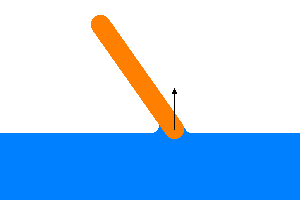
\includegraphics[width=1.3in]{figures/stages-of-a-plank-falling-into-water/1.png}
		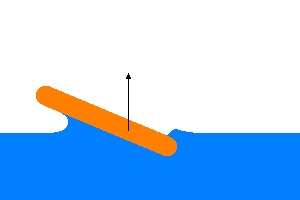
\includegraphics[width=1.3in]{figures/stages-of-a-plank-falling-into-water/2.png}
		
\includegraphics[width=1.3in]{figures/stages-of-a-plank-falling-into-water/3.png}
	\end{center}
	\caption{
		Stages of a plank falling into water.
		Black arrow indicates the net force applied on the plank.
	}
	\label{stages-of-a-plank-falling-into-water}
\end{figure}

Figure \ref{stages-of-a-plank-falling-into-water} shows a simple example demonstrating the complexity:
Assume that a piece of wood plank is falling into water at an angle.
When a side of it first touches the water, that side would immediately get pushed up, resulting in a torque causing the plank to pitch;
then the whole face of the plank will splat itself onto the water surface;
in the last, the plank's momentum is sufficiently decreased and it will slowly sink into or hold still on the water.
To simulate this whole process in a computer, there are two difficulties to be dealt with:

\begin{enumerate}
	\item It is not easy to find the exact volume of the submerged part of a solid object.

		To get the accurate buoyancy force, one would have to find which parts exactly are sunk in the water and keep making queries to the geometrical shape of the solid object.
		Unfortunately, common game engines only provides very limited interfaces on geometry information of physical bodies.
		As a workaround manually iterate through all the surfaces of the physical body's collision mesh, calculate each forces applied on the surfaces, and sum them up.
		This would be a linear performance cost relating to the amount of triangle surfaces of the floating object.
		The more complex the object's geometry is, the longer the algorithm needs to run.

	\item It could be overly computationally expensive or sometimes impossible.

		Finding only the accurate geometry information isn't enough, as every surfaces could be partially sunk in the water.
		If the algorithm only uses the full area of the surfaces to calculate the buoyancy force, then soon as an object touches the water, it would receive the maximum buoyancy force, which leads to artifacts.
		To avoid this, all surfaces of the mesh must clipped in each time the algoritm runs.
		Not only this would cause more performance cost, it also requires a clear, definite boundary of the water surface to be queried during runtime.
		As the implementation of the water body varies, this might even be impossible to achieve.
\end{enumerate}

However, although it is difficult to calculate the exact solutions directly, it is possible to use the Monte-Carlo method to statistically solve the problem at a cost of a configurable amount of error due to the randomness introduced by the method.